% PROGETTAZIONE E CODIFICA

\chapter{Progettazione e codifica}\label{chap:design}

\section {Progettazione architetturale}
\subsection{Architettura OpenChat}
Avendo dovuto basare l'applicazione Teamwork sulla soluzione già implementata per il web dalla zimlet OpenChat è utile approfondire la sua architettura.
\begin{figure}[H] 
	\centering
	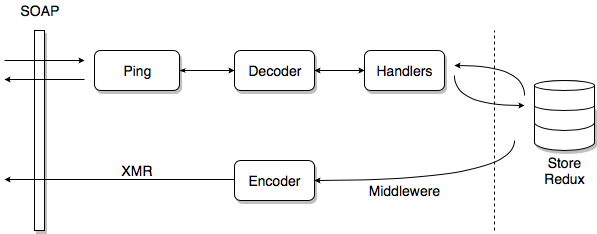
\includegraphics[scale=0.6]{architettura}
	\caption{Architettura OpenChat}
\end{figure}
La zimlet OpenChat interagisce con Zimbra grazie a delle connessioni SOAP. Questo permette la ricezione e l'invio di eventi anche da più sessioni contemporaneamente \mmh{e tutte sincronizzate tra di loro.}{, mantenendo tra loro la sincronizzazione/mantenendole sincronizzate}\\
Il connection manager si occupa della ricezione degli eventi:
\begin{itemize}
	\item il Ping serve a tenere aperta la connessione una volta creata e ad "ascolare" la connessione in modo da rendere reattiva l'applicazione alla ricezione degli eventi;
	\item \mmh{arrivato}{ricevuto?} un evento il decoder ha il compito di decodificarlo, trasformandolo da un file JSON ad una classe meglio gestibile.
\end{itemize}
Una volta ottenuto un evento tramite degli handlers sarà facilmente aggiornato lo store Redux con cui è gestita l'informazione lato front-end.

\note{ Modificare immagine, capire come mandano loro le informazioni}

\subsection{Modifiche architettura}
\note{cambiato un po' come arrivano gli eventi e tutto su come gli mando}

\section{Progettazione grafica}
Prima di procedere alla definizione delle classi necessarie per l'implementazione 
dell'applicazione è stato deciso di effettuare la progettazione \mmh{grafica della UI}{secondo me basta la progettazione della UI o la progettazione della grafica dell'app} per far 
si che il progetto di stage abbracciasse a 360 gradi il processo di sviluppo di 
un'applicazione da parte di un'azienda.

\subsection{Wireframe}
In base ai requisiti e agli use case raccolti è stato definito il modello iniziale
 dell'applicazione tramite la realizzazione dei wireframe delle varie schermate. \\
Questo studio è la prima rappresentazione visuale dell'applicazione ed ha lo 
scopo di identificare la struttura, l'architettura dell'informazione e la 
disposizione degli elementi nella pagina.\\
Di seguito vengono riportati i wireframe sviluppati di alcune delle pagine più 
importanti di Teamwork:
\begin{figure}[H] 
	\centering
	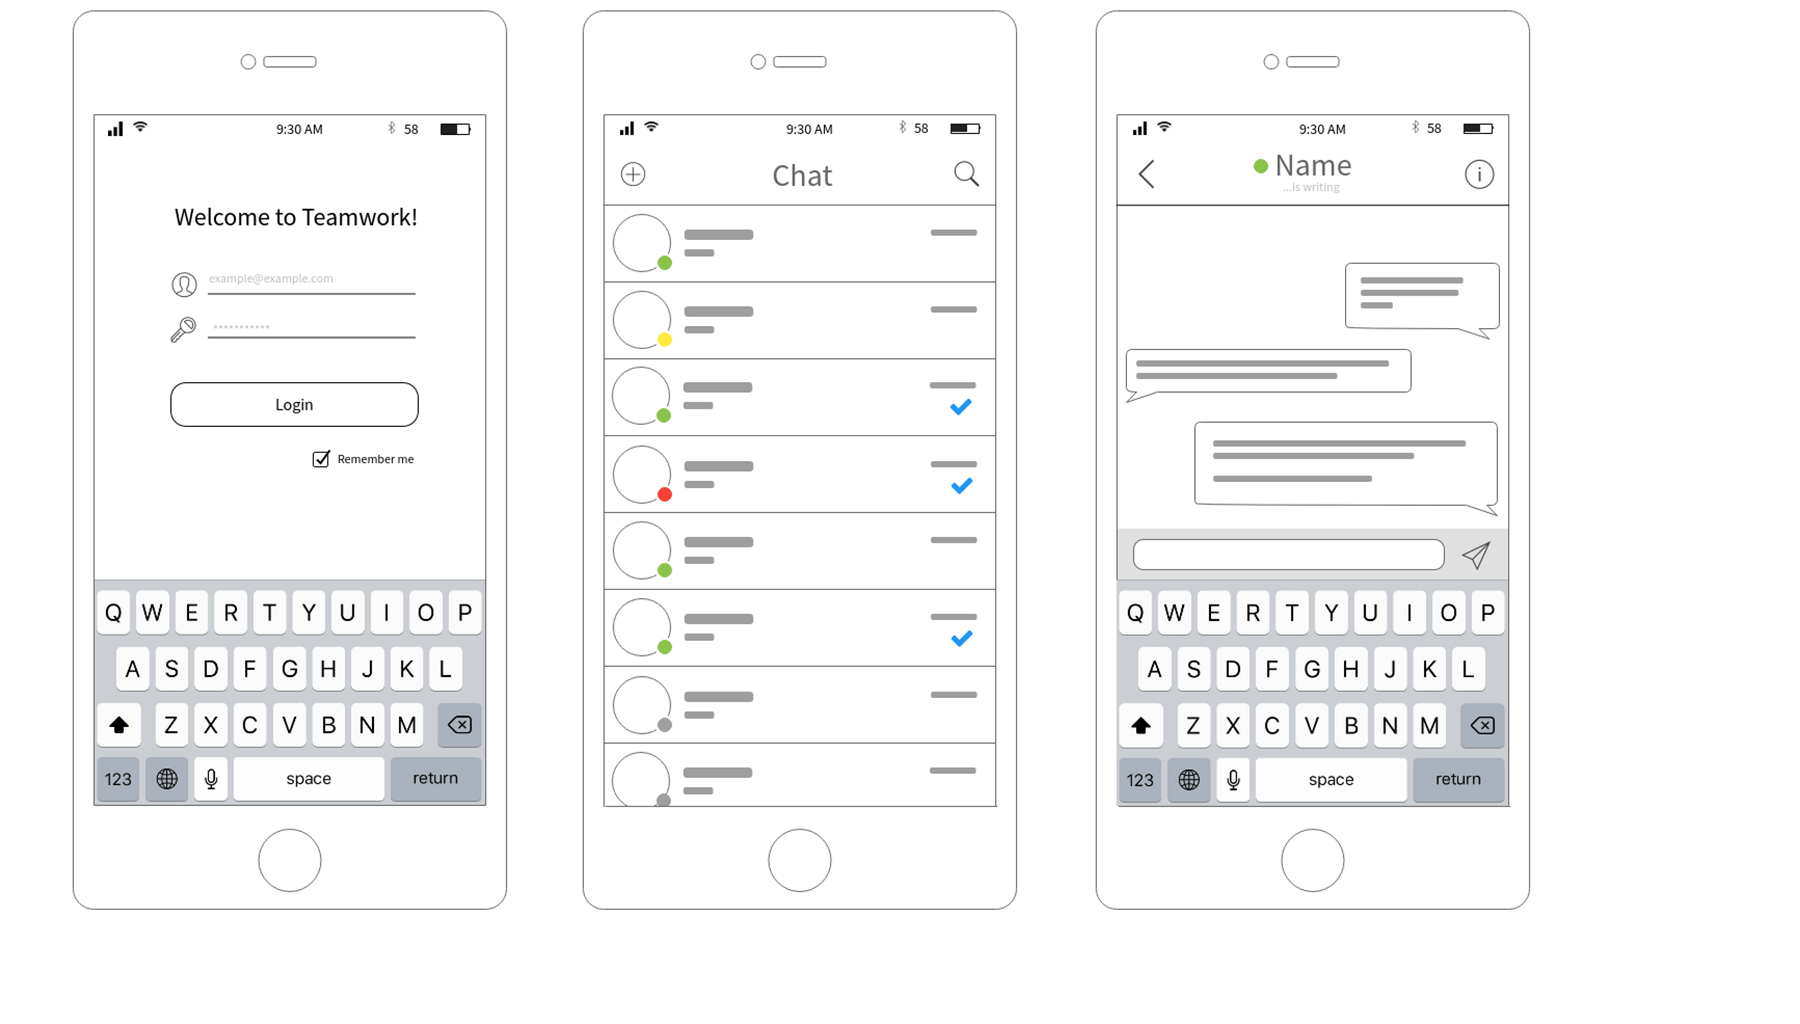
\includegraphics[scale=0.5]{wireframe}
	\caption{Wireframe pagina di login, buddylist e chat page.}
\end{figure}
Come possiamo notare dagli esempi riportati, in questa fase non è stato deciso 
nulla riguardo la rappresentazione grafica dei vari elementi. 
Si è definita soltanto la struttura delle varie schermate, il collegamento tra 
di esse e quali elementi realmente soddisfino i requisiti già studiati. 
Il risultato, comunque, è stato molto vicino alla GUI ottenuta alla fine della 
codifica in quando i wireframe sono stati disegnati tenendo conto della 
soluzione web già presente.\\ 
Questo passo è stato essenziale \mmh{per farsi un'idea più chiara di come proseguire per ottenere il risultato desiderato}{non mi piace, sembra troppo colloquiale, metterei tipo \emph{per rendere più chiara l'idea del prodotto desiderato.}}.

\subsection{Linee guida}
Per quanto riguarda la GUI vera e propria sono state fornite dall'azienda delle 
guidelines da seguire per la rappresentazione grafica di ogni elemento. \\
Nello specifico le guidelines toccano temi come:
\begin{itemize}
	\item le proporzioni tra i componenti;
	\item i colori da utilizzare;
	\item le definizioni di alcuni elementi base;
\end{itemize}
Questo serve per avere uno stile comune tra le varie applicazioni che 
l'azienda sviluppa. \\
Un esempio è la definizione del componente "card", destinato alla 
visualizzazione dei dettagli relativi ad un buddy:
\begin{figure}[H] 
	\centering
	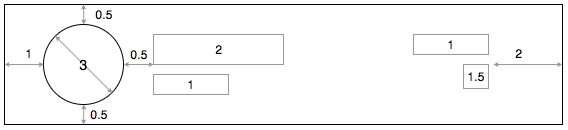
\includegraphics[scale=0.5]{guidelines}
	\caption{Esempio guidelines spazi}
\end{figure}
Si noti come ogni elemento sia posizionato in modo preciso definendo delle 
proporzioni tra gli spazi. In questo modo la successiva codifica dello stile sarà 
assolutamente definita da regole precise in modo da non dover interagire in modo 
continuativo con il responsabile grafico del progetto. \\
L'applicazione delle guidelines nel codice è avvenuta in parallelo con lo sviluppo 
in quando, seguendo una metodologia agile, si è ritenuto opportuno che le varie 
versioni prototipali dell'applicazione avessero anche una progressiva applicazione 
delle regole di stile.

\section{Progettazione di dettaglio}
Approvati i wireframe è stato possibile proseguire alla definizione di tutti 
e soli i componenti veramente utili al layout.